% !TEX root = msc_thesis.tex

\begin{figure}[tb]
	\centering
	\begin{subfigure}[t]{1\textwidth}
		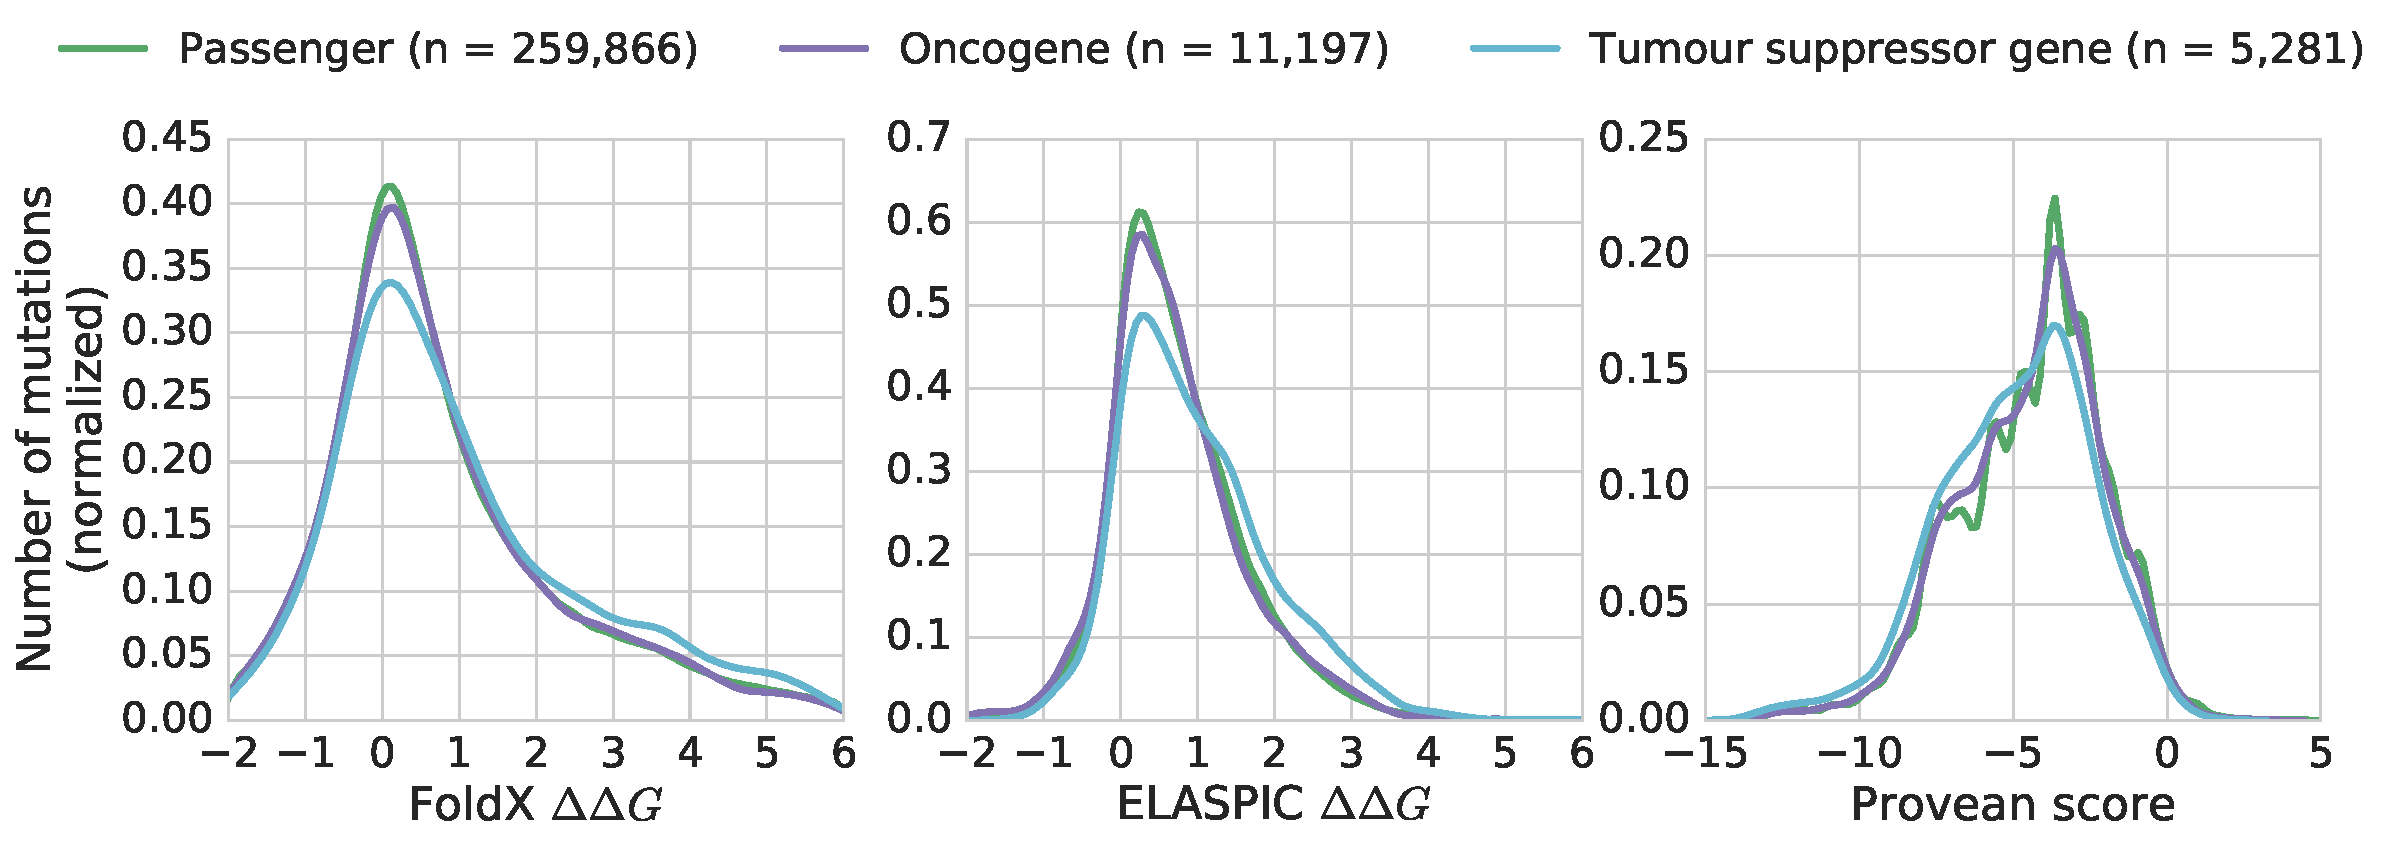
\includegraphics[width=1\linewidth]{static/elaspic_training_set/validation_cancer/score_distribution_full.pdf}
		\caption{
			Distribution of scores produced by FoldX (left), ELASPIC (middle) and Provean (right) for predicted cancer driver mutations in the COSMIC database. For all three programs, the scores obtained for mutations falling inside oncogenes are significantly different from the scores obtained for mutations falling inside tumour suppressor genes, according to the Mann--Whitney U test (FoldX p-value $< 1 \times 10^{-18}$, ELASPIC p-value: $< 1 \times 10^{-56}$, Provean p-value: $< 1 \times 10^{-25}$).
		}
		\label{fig:validation_cancer_score_distribution_full}
		\vspace*{10mm}
	\end{subfigure}

	\begin{subfigure}[t]{1\textwidth}
		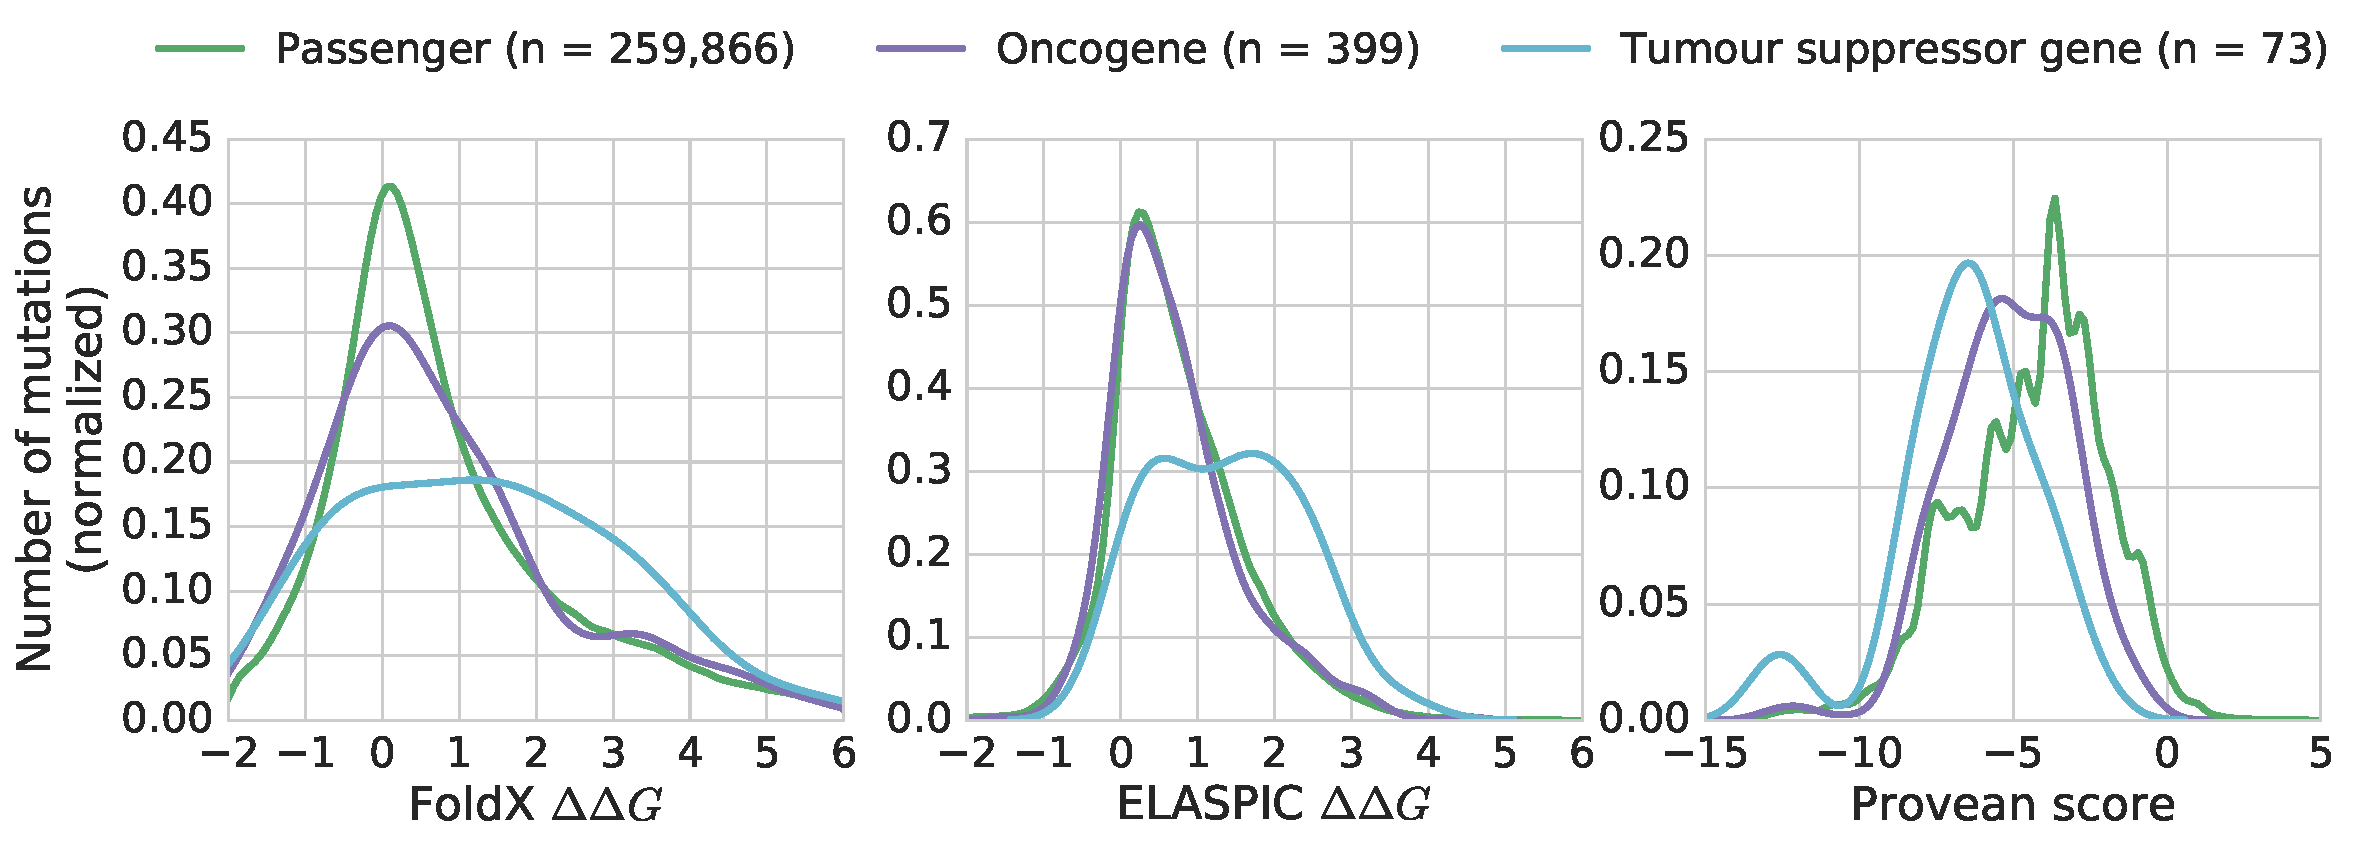
\includegraphics[width=1\linewidth]{static/elaspic_training_set/validation_cancer/score_distribution_high_confidence.pdf}
		\caption{
		Distribution of scores produced by FoldX (left), ELASPIC (middle) and Provean (right) for currated cancer driver mutations in DoCM. For ELASPIC and Provean, the scores obtained for mutations falling inside oncogenes are significantly different from the scores obtained for mutations falling inside tumour suppressor genes, according to the Mann--Whitney U test (FoldX p-value $> 0.05$, ELASPIC p-value: $< 1 \times 10^{-7}$, Provean p-value: $< 1 \times 10^{-5}$).
		}
		\label{fig:validation_cancer_score_distribution_high_confidence}
		\vspace*{5mm}
	\end{subfigure}

	\caption[Distribution of scores for mutations in oncogenes and tumour suppressor genes.]{
			Distribution of scores produced by FoldX, ELASPIC and Provean for mutations in the COSMIC database predicted to be cancer drivers by FATHMM (a) and for mutations in the database of curated mutations (DoCM) known to be cancer drivers through \textit{in vitro} and \textit{in vivo} experiments.
		}
	\label{fig:validation_cancer_score_distribution}
\end{figure}


\clearpage


\begin{figure}[tb]
	\centering
	\begin{subfigure}[t]{0.48\textwidth}
		\centering
		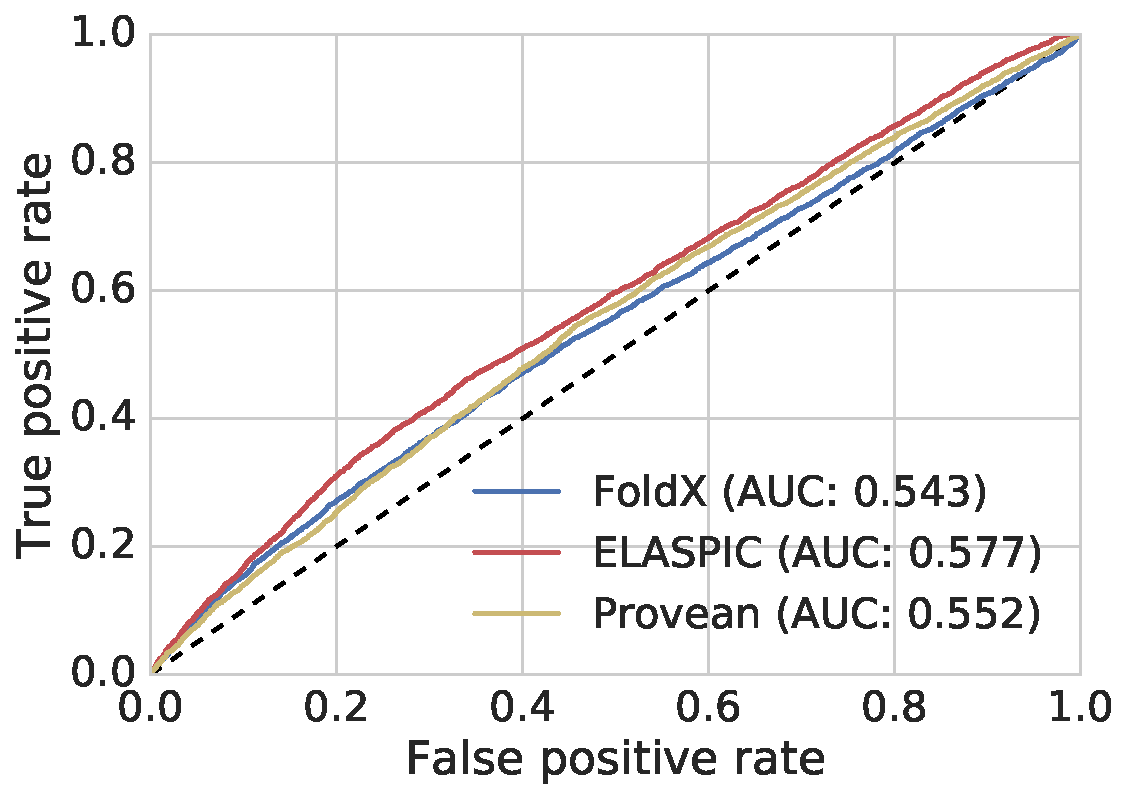
\includegraphics[width=1\linewidth]{static/elaspic_training_set/validation_cancer/roc_curve_full.pdf}
		\caption{
			Predicting whether a \textit{mutation} falls inside an oncogene or a tumour suppressor gene, for all deleterious mutations in COSMIC.
		}
		\label{fig:validation_cancer_full}
		\vspace*{10mm}
	\end{subfigure}%
	\hspace*{5mm}
	\begin{subfigure}[t]{0.48\textwidth}
		\centering
		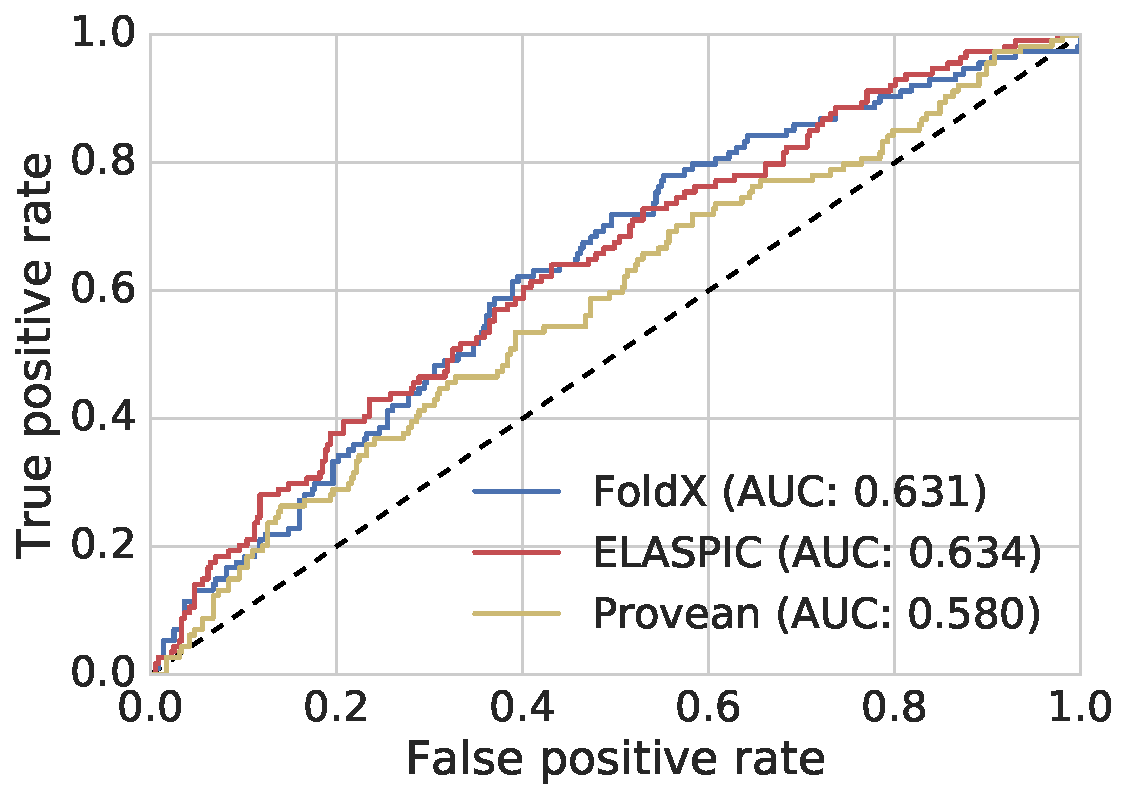
\includegraphics[width=1\linewidth]{static/elaspic_training_set/validation_cancer/roc_curve_bygene_full.pdf}
		\caption{
			Predicting whether a \textit{protein} is an oncogene or a tumour suppressor gene, using all deleterious mutations in the COSMIC database.
		}
		\label{fig:validation_cancer_bygene_full}
		\vspace*{10mm}
	\end{subfigure}

	\begin{subfigure}[t]{0.48\textwidth}
		\centering
		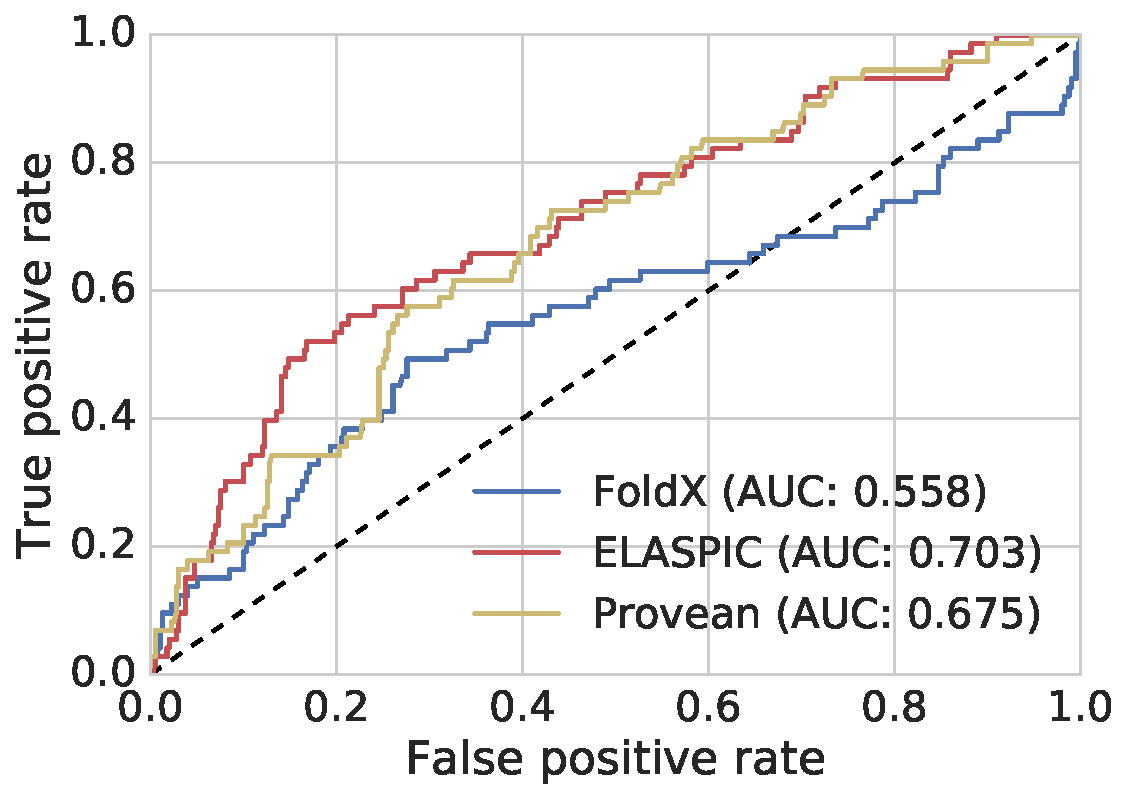
\includegraphics[width=1\linewidth]{static/elaspic_training_set/validation_cancer/roc_curve_high_confidence.pdf}
		\caption{
			Predicting whether a \textit{mutation} falls inside an oncogene or a tumour suppressor gene, for all deleterious mutations in DoCM \cite{griffith_civic:_2016}.
		}
		\label{fig:validation_cancer_high_confidence}
		\vspace*{5mm}
	\end{subfigure}%
	\hspace*{5mm}
	\begin{subfigure}[t]{0.48\textwidth}
		\centering
		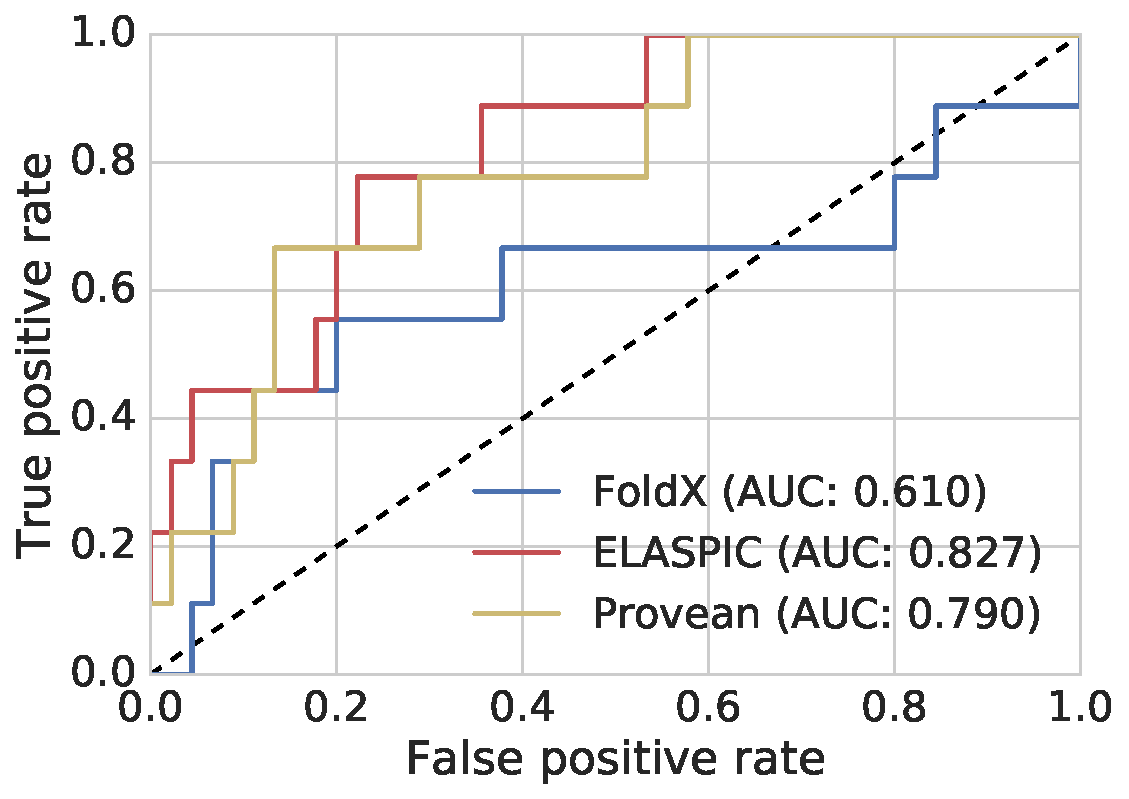
\includegraphics[width=1\linewidth]{static/elaspic_training_set/validation_cancer/roc_curve_bygene_high_confidence.pdf}
		\caption{
			Predicting whether a \textit{protein} is an oncogene or a tumour suppressor gene, using all deleterious mutations in DoCM \cite{griffith_civic:_2016}.
		}
		\label{fig:validation_cancer_bygene_high_confidence}
		\vspace*{5mm}
	\end{subfigure}%
	\caption[Predicting whether a mutation falls in an oncogene or a tumour suppressor gene.]{
			Receiver operating characteristic (ROC) curves showing the performance of FoldX, ELASPIC and Provean in predicting whether a \textit{mutation} falls inside an oncogene or a tumour suppressor gene (a, c), or whether the \textit{entire protein} is an oncogene or a tumour suppressor gene (b, d), using all deleterious mutations in the COSMIC database (a, b) or curated driver mutations in the DoCM database \cite{griffith_civic:_2016} (c, d).
			When predicting whether the entire protein is an oncogene or a tumour suppressor gene, we used the mean score for all mutations falling in that protein.
		}
	\label{fig:validation_cancer}
\end{figure}
